\section{Methodology and Implementation}

	\subsection{Research Strategy and Approach}
	\noindent Before receiving the dataset, I have conducted an exhaustive investigation of the clinical landscape surrounding hypoglycaemia as a health condition, including studying the situations in which it commonly occurs, both in hospital settings as well as in public or everyday life. I have scrutinized a plethora of factors contributing to hypoglycaemia, including associated medicines (even conflicting medications), at-risk patient profiles, habits and lifestyles, dosing errors (both excessive as well as insufficient (\textit{insulin})), missed meals and even alcohol consumption. This has allowed me to better assess the quality of the incoming dataset and the relevance of its features. Upon requesting additional information regarding current patient medication and alcohol intake as it was not provided originally, GSTT advised that this data is unavailable because of its inconsistent self-reported nature and due to restrictions under their information governance policy that permits access to only the data deemed necessary for the project's scope.

	\vspace{10pt}
	\noindent After receiving the data, I have thoroughly \textbf{preprocessed} it to ensure it was suitable for meaningful analysis. This included addressing data type mismatches, deriving variables to aid in visualisation and understanding, and performing necessary imputations using appropriate methods. Duplicate and missing records were handled, categorical variables were encoded to make them compatible for predictive modelling, data validity and consistency checks were enacted to confirm that values were in expected ranges (for e.g. the glucose value field), normalization was carried out where necessary. These steps were necessary to lay a strong foundation for the subsequent application of statistical tests and machine learning models. The full preprocessing workflow is depicted in \autoref{fig:datapreprocessingwf} below. \
	
	\vspace{10pt}
	\noindent Following this, my focus was on \textbf{exploratory data analysis} to spot any anomalies or patterns near the surface. After devising research questions around the dataset, I have generated a collection of plots through Python's widely used seaborn library that I describe in detail in \hyperref[sec:mainResults]{the main results section}, which shed light on the prevalence of hypoglycaemia across various different scenarios. Special attention was paid to drawing comparisons between hypoglycaemic and non hypoglycaemic patients, in alignment with GSTT's interests that they had clarified in the project's early stages.

	\begin{figure}[H]
		\centering
		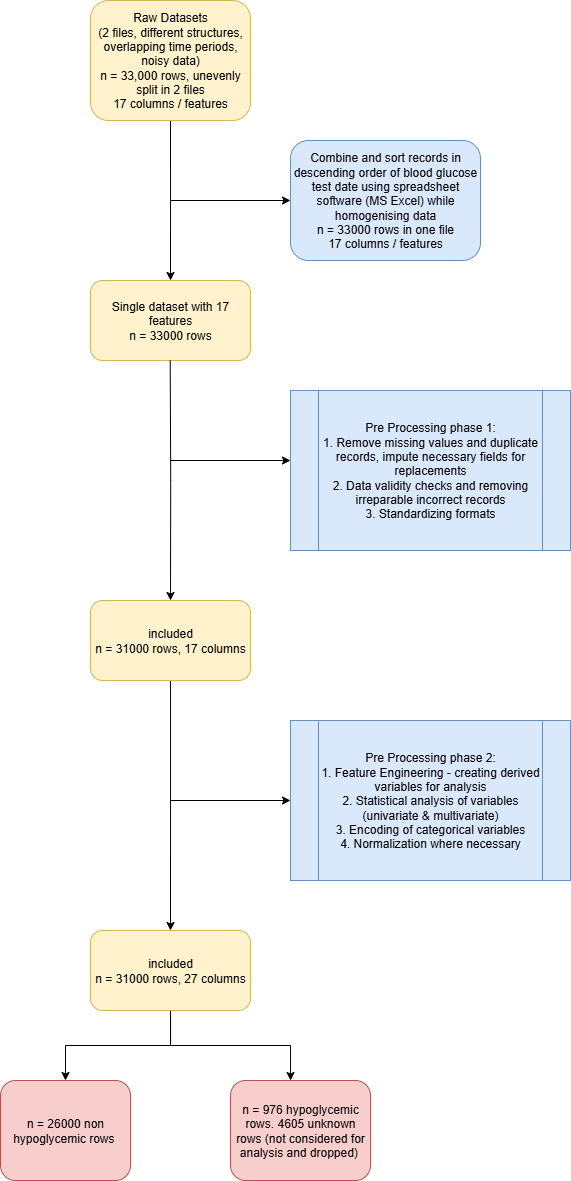
\includegraphics[height=8in]{figures/dataPreprocessingWf.png}
		\caption{Data preprocessing workflow}
		\label{fig:datapreprocessingwf}
	\end{figure}

	\subsection{Dealing With Imbalanced Data}
	\noindent It was found that there is a considerable imbalance between the number of hypoglycaemic patients (976) vs the non-hypoglycaemic patients(26022) through preprocessing. Considering this imbalance, no augmentation or sampling techniques have been carried out in the initial stages of this project to preserve the integrity and objectivity of the exploratory data analysis (EDA) phase. The rationale behind this decision was to ensure that any findings discovered from this effort remained reflective of the raw data as originally provided. Introducing synthetic data points at this stage would have led to skewed or misleading statistical and visual conclusions, especially when it comes to comparative sub-group analysis. Exploratory data analysis on a pure unadulterated dataset enabled me to locate and assess disparities between hypoglycaemic and non-hypoglycaemic patients with full clarity free from any distortion. I have visualised and documented these in the form of answers to research questions. This enabled me to meet the first objective of the project of generating benefical, usable insights from the data without any ambiguity as to how they had been obtained.

	\vspace{5pt}
	\noindent In the predictive modelling stage of the project, some conditional sampling has been selectively employed, so as to maximise model performance. The rationale behind this was to ensure that the training process remained robust and was not biased towards the majority class. \textbf{Conditional Sampling} is a data manipulation technique where data points are drawn from a subset of a larger dataset that has been filtered on the basis of certain conditions to yield those data points that match a certain range or pattern. This yields better quality rows as compared to random sampling, and the exemplars so picked from conditional sampling were varied to not be identical to other ones. Care was taken in doing so to apply these techniques, so as to only produce sensible and valid values, in a manner so as to not undermine earlier findings. \textbf{A dual phased approach such as this one provided a healthy balance between data integrity in the early exploratory stages as well as enhanced performance in the later predictive modelling stages. }

	\subsection{Machine Learning Theories}
	
	\noindent With findings and observations from the exploratory data analysis process now established, I directed attention to the second major project objective.  To devise a risk score for hypoglycaemia, I would first need to identify the principal components from the dataset, that is to say the features that most influence hypoglycaemia or contribute to its presence. Following this, I would need to find the values of those features which are "turning points" or at which a decision is made (for example, the "turning point" for the "age" feature would be in the higher range as old age invites complications, so this could be something from 70-90 years). This has been completed through both the EDA phase as well as some statistical and machine learning techniques that I have detailed further.

	\subsubsection{Decision Trees}
	The rationale behind using Decision Trees was that it is the most suitable algorithm to find the thresholds of the key predictors of hypoglycaemia(like HbA1c). A Decision Tree is a supervised learning algorithm that can be used for both classification and regression, matching our objective of predicting hypoglycaemia through a risk score. Its structure is hierarchical resembling a flowchart where each internal node represents a test on a feature, every branch represents the outcome of that test, and each leaf node represents the final decision or the class label. It functions by learning a set of interpretable rules from the dataset features. 

	\vspace{5pt}
	\noindent The algorithm works by a process called recursive partitioning. The process begins at the root node, which contains the entire patient dataset in our case (both hypoglycaemic and non-hypoglycaemic patients). The algorithm then looks at each input feature one by one (HbA1c, eGFR etc.) and systematically test every possible value of that input feature for being a potential split point. It determines the best "split" by a metric known as \textbf{Gini's Impurity Index} which measures the probability of incorrectly classifying a randomly chosen patient from one of the 2 hypoglycaemic groups. The algorithm strives to minimise this value (A score of 0 is ideal meaning perfect purity), meaning that the resulting child nodes from the split are "pure" and contain no misclassified samples. Considering a dataset $D$ with samples from $k$ classes, Gini Impurity is calculated as follows: 
	
	$$ Gini(D) = 1 - \sum_{i=1}^{k} p_{i}^2	$$

	\noindent Where: 
	\begin{itemize}
		\item $D$ is the dataset containing samples from $k$ classes 
		\item $p_{i}$ is the probability of samples belonging to class $i$ at a given node
	\end{itemize}
			
	\vspace{5pt}
	\noindent The algorithm then compares purity scores from all the potential splits across all the features. It will select the single feature and the specific value of that feature that results in the most purity (and therefore creates the best possible split). 

	\vspace{5pt}
	\noindent Applying this to our own dataset, to determine the decision point for a feature like HbA1c for example, the algorithm would work like so: 
	\begin{itemize}
		\item Let's assume the observed values range from 40 to 100. The algorithm will test splits like $HbA1c > 40$, $HbA1c > 41$ and so on
		\item For each of these potential splits it calculates the impurity of the resulting 2 subsets of patients $i.e.$ those above that current HbA1c threshold and those below it
		\item The specific HbA1c value that yields the lowest Gini Impurity value is then selected as the optimal decision rule for that node. We can then assert that HbA1c becomes most discriminative (most influential) for predicting hypoglycaemia risk at this empirically derived value, and this is how we arrive at the most discriminative values for the main predictors of hypoglycaemia. 
	\end{itemize}

	\vspace{5pt}
	\noindent The feature and threshold selected at the root node split is considered to be the most powerful predictor in the dataset. However, with Decision Trees, it is vital to \textbf{avoid overfitting} which is where the tree ends up capturing or considering noise instead of the true behaviour / nature of the data. This can be managed by pruning (cutting short) the tree, or setting hyperparameters like $max_depth$, but as a step up I have employed Random Forest algorithm which works by aggregating multiple Decision Trees to get the best result.  

	\subsubsection{Random Forest}
	Random Forest is an ensemble learning algorithm that works by building a large number of individual decision trees and then combining their outputs to make a final prediction. It is advantageous over regular decision trees as it is resistant to overfitting and as errors or biases in the model average out, it tends to produce a more stable collective result. Furthemore, by measuring how much a feature like HbA1c contributes to reducing impurity across all the trees that the model creates, the model can produce a feature importance score enabling us to rank the predictors in the dataset based on their significance or value.
	\begin{itemize}
		\item To start with, the algorithm conjures up many different training sets by repeatedly drawing random samples from the original dataset with replacement, meaning that some data points may be selected more than once and some may not be selected at all. Each individual decision tree is then trained on one of these unique randomly built datasets, hence the name "Random" for random sampling and "Forest" meaning multiple Decision Trees. This process is also called Bagging or Bootstrap Aggregation.
		\item As each tree is being built, it is not allowed to use all the available information to make its decisions. The tree is only given a random subset of the total features (e.g., only 3 out of 10 patient attributes) to choose from at every split point. This forces the forest to learn from a wider variety of predictors in addition to preventing any single strong feature from dominating all the trees.
		\item Once all the trees in the forest have been built, every tree in the forest makes a prediction when a new unseen data point comes along. The final prediction outcome from the Random Forest model is simply the one that received the most votes from all the trees, and this collective majority voting makes the final result more accurate as well as less error-prone. 
	\end{itemize}

	\vspace{5pt}
	\noindent Despite being more powerful than a single Decision Tree, it is still a formidable challenge to choose the optimal number and values of hyperparameters for a Random Forest, such as the number of trees to build or the max depth of each tree. To tackle this problem we harness the power of GridSearchCV to find the best hyperparameters to build a Random Forest.
	
	\subsubsection{GridSearchCV}
	GridSearchCV stands for Grid Search Cross Validation. GridSearchCV is valuable and advantageous because it takes a methodical and exhaustive approach ("try everything out and find the best") to ascertain the optimal values of hyperparameters. Choosing the right values of hyperparameters to train a Random Forest is crucial because it can lead to a model that is either too simple and underfits or too complex and overfits, GridSearchCV enables us to address this issue. Its name breaks down its process:
	\begin{itemize}
		\item \textbf{Grid:} We define a "grid" of hyperparameters and their values to try. For example a grid could have $max\_depth$ values of [3,5,7] and $n\_estimators$ (number of trees to build) of [50,100,125] in the grid.
		\item \textbf{Cross Validation:} GridSearchCV splits the training data into ``folds'' and for each hyperparameter combination, it trains the model on some folds and tests it on the remaining folds, while continuously rotating around which fold is used for testing with every iteration. Finally it averages the performance scores from all the folds. 
	\end{itemize}

	GridSearchCV is highly beneficial in that it automates what would have been a very tedious manual task while also producing the best possible reliable results and reducing the risk of overfitting. Although it does return the best possible hyperparameter values to train the model, there is a risk of making the "grid" too large, which could potentially lead to GridSearchCV running for ages, sometimes even days or  weeks, so it is imperative to choose an accurately sized grid based on the data and objective at hand.

	% Decision tree
	% random forest 
	% grid search cv 
	% conditional sampling 
	% xgboost

	% It presents and justifies the methodology used to deal with the problem and describes in detail the implementation procedures. The background theory presented in the previous chapter can be recalled to support the proposed implementation. The originality, novelty and contribution are to be demonstrated with the discussion of the strengths and limitations.